% Source PDF page 315 (printed p. 301)
\subsection{带约束的逼近}
可以在基本范数逼近问题 (6.1) 中加入约束。若这些约束是凸的，所得到的问题也是凸问题。约束可能出于多种原因。
\begin{itemize}
\item 在逼近问题中，可以用约束排除某些不可接受的向量 $b$ 的近似，或者保证逼近向量 $Ax$ 满足某些性质。
\item 在估计问题中，约束来自对待估向量 $x$ 的先验知识，或者对估计误差 $v$ 的先验知识。
\item 在几何问题中，要确定点 $b$ 在比子空间更复杂的集合（例如锥或多面体）上的投影，也会产生约束。
\end{itemize}
下面用几个例子说明。

\subsubsection*{变量的非负约束}
在基本范数逼近问题中加入约束 $x\succeq0$：
\[\begin{array}{ll}\text{最小化}&\norm{Ax-b}\\\text{约束条件}&x\succeq0.\end{array}\]
在估计中，如果已知待估参数向量 $x$ 的分量非负，例如功率、强度或速率，就会有非负约束。几何上，这是确定向量 $b$ 到由 $A$ 的列生成的锥的投影。也可以把该问题解释为用 $A$ 的列的非负线性组合（即锥组合）逼近 $b$。

\subsubsection*{变量界}
这里加入约束 $l\preceq x\preceq u$，其中 $l,u\in\R^n$ 是问题参数：
\[\begin{array}{ll}\text{最小化}&\norm{Ax-b}\\\text{约束条件}&l\preceq x\preceq u.\end{array}\]
在估计中，变量界来自预先知道的各变量所在区间。几何上，这是求向量 $b$ 到一个盒在由 $A$ 定义的线性映射下的像的投影。

% Source PDF page 316 (printed p. 302)
\subsubsection*{概率分布}
可以要求 $x$ 满足 $x\succeq0$、$\one^\T x=1$：
\[\begin{array}{ll}\text{最小化}&\norm{Ax-b}\\\text{约束条件}&x\succeq0,\quad\one^\T x=1.\end{array}\]
在估计比例或相对频率时会有这样的约束，因为它们非负且总和为 $1$。这也可以解释为用 $A$ 的列的凸组合逼近 $b$。（第7.2节将详细讨论概率估计。）

\subsubsection*{范数球约束}
可以在基本范数逼近问题中加入 $x$ 位于某个范数球内的约束：
\[\begin{array}{ll}\text{最小化}&\norm{Ax-b}\\\text{约束条件}&\norm{x-x_0}\le d,\end{array}\]
其中 $x_0$ 和 $d$ 是问题参数。加入这一约束有以下几种理由。
\begin{itemize}
\item 在估计中，$x_0$ 是对参数 $x$ 的先验猜测，$d$ 是我们认为估计相对于先验猜测可能偏离的最大幅度。参数 $x$ 的估计值 $\widehat x$，是在所有可信候选值（满足 $\norm{z-x_0}\le d$ 的 $z$）中，与测量数据最匹配的值，即使 $\norm{Az-b}$ 最小的值。
\item 约束 $\norm{x-x_0}\le d$ 可以表示一个\emph{信赖域}。这里，线性关系 $y=Ax$ 只是某个非线性关系 $y=f(x)$ 的近似；仅当 $x$ 靠近某点 $x_0$，具体说满足 $\norm{x-x_0}\le d$ 时，这一近似才成立。问题要在模型 $y=Ax$ 可信的那些 $x$ 中最小化 $\norm{Ax-b}$。
\end{itemize}
这些想法也会在正则化中出现，见第6.3.2节。

\section{最小范数问题}
基本的最小范数问题为
\begin{equation}
\begin{array}{ll}\text{最小化}&\norm x\\\text{约束条件}&Ax=b,\end{array}\tag{6.5}
\end{equation}
其中数据为 $A\in\R^{m\times n}$、$b\in\R^m$，变量为 $x\in\R^n$，$\norm{\cdot}$ 是 $\R^n$ 上的一个范数。只要线性方程 $Ax=b$ 有解，该问题的解就一定存在，称为 $Ax=b$ 的\emph{最小范数解}。最小范数问题当然是凸优化问题。

不失一般性，可以假设 $A$ 的行线性无关，因此 $m\le n$。当 $m=n$ 时，唯一可行点为 $x=A^{-1}b$；只有当 $m<n$，即方程 $Ax=b$ 是欠定方程时，最小范数问题才有意义。

% Source PDF page 317 (printed p. 303)
\subsubsection*{改写为范数逼近问题}
通过消去等式约束，可以将最小范数问题 (6.5) 写成范数逼近问题。令 $x_0$ 为 $Ax=b$ 的任意一个解，$Z\in\R^{n\times k}$ 的列构成 $A$ 的零空间的一组基。那么，$Ax=b$ 的通解为 $x_0+Zu$，其中 $u\in\R^k$。最小范数问题 (6.5) 可以写成
\[\text{最小化}\quad\norm{x_0+Zu},\]
变量为 $u\in\R^k$；这是一个范数逼近问题。特别地，对范数逼近问题的分析与讨论，作适当解释后，也同样适用于最小范数问题。

\subsubsection*{控制或设计解释}
最小范数问题 (6.5) 可以解释为最优设计或最优控制问题。$n$ 个变量 $x_1,\ldots,x_n$ 是待确定取值的设计变量。在控制中，这些变量表示要选择取值的输入。向量 $y=Ax$ 给出设计 $x$ 的 $m$ 个属性或结果，假定它们是设计变量 $x$ 的线性函数。$m<n$ 个方程 $Ax=b$ 表示对设计的 $m$ 项指标或要求。由于 $m<n$，这些要求尚未完全确定设计；设计中还有 $n-m$ 个自由度（假设 $A$ 的秩为 $m$）。

在所有满足指标的设计中，最小范数问题选择按 $\norm{\cdot}$ 衡量最小的设计。这可以看作最高效的设计：它用尽可能小的 $x$ 达到指标 $Ax=b$。

\subsubsection*{估计解释}
假设 $x$ 是待估计的参数向量。我们有 $m<n$ 个完全精确、没有噪声的线性测量 $Ax=b$。由于测量数少于待估参数数，测量不能完全确定 $x$。任何满足 $Ax=b$ 的参数向量 $x$ 都与测量一致。

要在不增加测量的情况下合理猜测 $x$，必须使用先验信息。假设先验信息或假设是：按 $\norm{\cdot}$ 衡量，$x$ 更可能较小而非较大。最小范数问题就在所有与测量 $Ax=b$ 一致的参数向量中，选择最小、因而最可信的一个作为估计。（最小范数问题的统计解释见第359页。）

\subsubsection*{几何解释}
最小范数问题 (6.5) 也有一个简单的几何解释。可行集 $\{x\mid Ax=b\}$ 是仿射集，目标是 $x$ 到原点的距离（以 $\norm{\cdot}$ 衡量）。最小范数问题寻找该仿射集中距离原点最近的点，即确定原点到仿射集 $\{x\mid Ax=b\}$ 的投影。

% Source PDF page 318 (printed p. 304)
\subsubsection*{线性方程的最小二乘解}
最常见的最小范数问题使用欧几里得范数，即 $\ell_2$ 范数。将目标平方，得到等价问题
\[\begin{array}{ll}\text{最小化}&\norm x_2^2\\\text{约束条件}&Ax=b,\end{array}\]
其唯一解称为方程 $Ax=b$ 的\emph{最小二乘解}。与最小二乘逼近问题一样，该问题也可解析求解。引入对偶变量 $\nu\in\R^m$，最优性条件为
\[2x^\star+A^\T\nu^\star=0,\qquad Ax^\star=b,\]
这是一组容易求解的线性方程。从第一个方程得到 $x^\star=-(1/2)A^\T\nu^\star$，代入第二个方程得到 $-(1/2)AA^\T\nu^\star=b$，从而
\[\nu^\star=-2(AA^\T)^{-1}b,\qquad x^\star=A^\T(AA^\T)^{-1}b.\]
（由于 $\rank A=m<n$，矩阵 $AA^\T$ 可逆。）

\subsubsection*{最小惩罚问题}
最小范数问题 (6.5) 的一种有用变体是\emph{最小惩罚问题}
\begin{equation}
\begin{array}{ll}\text{最小化}&\phi(x_1)+\cdots+\phi(x_n)\\\text{约束条件}&Ax=b,\end{array}\tag{6.6}
\end{equation}
其中 $\phi:\R\to\R$ 是凸且非负的函数，并满足 $\phi(0)=0$。惩罚函数值 $\phi(u)$ 量化我们对 $x$ 的某个分量取值为 $u$ 的不满意程度；最小惩罚问题则在约束 $Ax=b$ 下，寻找总惩罚最小的 $x$。

惩罚函数逼近中关于惩罚函数的全部讨论与解释，都可以移用于最小惩罚问题，只需将惩罚逼近问题中残差 $r$ 的幅度分布，换成最小惩罚问题中 $x$ 的幅度分布。

\subsubsection*{用最小 $\ell_1$ 范数获得稀疏解}
回顾第300页的讨论，$\ell_1$ 范数逼近对小残差赋予较大相对权重，因此许多最优残差会很小，甚至为零。最小范数问题中也会出现类似现象。最小 $\ell_1$ 范数问题
\[\begin{array}{ll}\text{最小化}&\norm x_1\\\text{约束条件}&Ax=b\end{array}\]
往往产生有大量零分量的解 $x$。换言之，最小 $\ell_1$ 范数问题倾向于产生 $Ax=b$ 的稀疏解，非零分量常有 $m$ 个。

% Source PDF page 319 (printed p. 305)
很容易找到只有 $m$ 个非零分量的 $Ax=b$ 的解。从 $1,\ldots,n$ 中任选 $m$ 个指标，作为 $x$ 的非零分量所在位置。方程 $Ax=b$ 就化为 $\widetilde A\widetilde x=b$，其中 $\widetilde A$ 是从 $A$ 中取相应列得到的 $m\times m$ 子矩阵，$\widetilde x\in\R^m$ 是由选定的 $m$ 个分量构成的 $x$ 的子向量。若 $\widetilde A$ 非奇异，可取 $\widetilde x=\widetilde A^{-1}b$，得到一个非零分量不超过 $m$ 个的可行解 $x$。若 $\widetilde A$ 奇异且 $b\notin\mathcal R(\widetilde A)$，则 $\widetilde A\widetilde x=b$ 无解，意味着在选定的非零位置上没有可行的 $x$。若 $\widetilde A$ 奇异且 $b\in\mathcal R(\widetilde A)$，则存在非零分量少于 $m$ 个的可行解。

这种方法可以寻找具有 $m$ 个或更少非零分量的最小 $x$，但通常需要检查并比较从 $x$ 的 $n$ 个系数中选择 $m$ 个非零系数的全部 $n!/[m!(n-m)!]$ 种可能。相比之下，求解最小 $\ell_1$ 范数问题，是寻找 $Ax=b$ 的稀疏且较小的解的一种良好启发式方法。

\section{正则化逼近}
\subsection{双准则表述}
正则化逼近的基本目标，是寻找一个尽可能小、同时也使残差 $Ax-b$ 小的向量 $x$。自然地，这可以表述为一个具有 $\norm{Ax-b}$ 和 $\norm x$ 两个目标的凸向量优化问题：
\begin{equation}
\text{相对于 }\R_+^2\text{ 最小化}\quad(\norm{Ax-b},\norm x).\tag{6.7}
\end{equation}
两个范数可以不同：第一个定义在 $\R^m$ 上，衡量残差大小；第二个定义在 $\R^n$ 上，衡量 $x$ 的大小。

两个目标之间的最优权衡可以通过多种方法求得，然后绘出 $\norm{Ax-b}$ 与 $\norm x$ 的最优权衡曲线；它表明，要使一个目标较小，另一个目标至少必须多大。$\norm{Ax-b}$ 与 $\norm x$ 的最优权衡曲线的一个端点容易描述。$\norm x$ 的最小值是零，仅在 $x=0$ 时取得；此时残差范数为 $\norm b$。

权衡曲线的另一个端点较复杂。令 $C$ 表示 $\norm{Ax-b}$ 的最小化点集合（对 $\norm x$ 不加约束）。那么，$C$ 中任意一个最小范数点都是 Pareto 最优点，对应权衡曲线的另一个端点。也就是说，这个端点对应的 Pareto 最优点，是使 $\norm{Ax-b}$ 最小的所有点中的最小范数点。如果两个范数都是欧几里得范数，该 Pareto 最优点唯一，为 $x=A^\dagger b$，其中 $A^\dagger$ 是 $A$ 的伪逆。（见第4.7.6节，第184页，以及第A.5.4节。）

% Source PDF page 320 (printed p. 306)
\subsection{正则化}
\emph{正则化}是求解双准则问题 (6.7) 常用的一种标量化方法。一种正则化形式是最小化两个目标的加权和：
\begin{equation}\text{最小化}\quad\norm{Ax-b}+\gamma\norm x,\tag{6.8}\end{equation}
其中 $\gamma>0$ 是问题参数。当 $\gamma$ 在 $(0,\infty)$ 上变化时，问题 (6.8) 的解描绘出最优权衡曲线。

另一种常用正则化方法，尤其在使用欧几里得范数时，是对不同的 $\delta>0$，最小化范数平方的加权和，即
\begin{equation}\text{最小化}\quad\norm{Ax-b}^2+\delta\norm x^2.\tag{6.9}\end{equation}
这些正则化逼近问题通过增加一个与 $x$ 的范数有关的附加项或惩罚项，求解同时使 $\norm{Ax-b}$ 和 $\norm x$ 较小的双准则问题。

\subsubsection*{解释}
正则化用于多种场合。在估计中，惩罚较大 $\norm x$ 的附加项可以解释为：先验知识认为 $\norm x$ 不会太大。在最优设计中，附加项把使用较大设计变量所带来的代价，加入偏离目标指标的代价。

要求 $\norm x$ 较小，也可能来自建模问题。例如，$y=Ax$ 可能只是 $x$ 与 $y$ 的真实关系 $y=f(x)$ 的良好近似。要有 $f(x)\approx b$，既希望 $Ax\approx b$，也需要 $x$ 较小，以保证 $f(x)\approx Ax$。

第6.4.1节和第6.4.2节将说明，正则化可以用来考虑矩阵 $A$ 的变化。粗略地说，较大的 $x$ 会使 $A$ 的变化导致 $Ax$ 的较大变化，因此应避免。

当矩阵 $A$ 是方阵、目标是求解线性方程 $Ax=b$ 时，也可以采用正则化。如果 $A$ 病态甚至奇异，正则化就在解方程（使 $\norm{Ax-b}$ 为零）与把 $x$ 保持在合理大小之间作出折中。

正则化也会出现在统计问题中；见第7.1.2节。

\subsubsection*{Tikhonov 正则化}
最常见的正则化形式基于式 (6.9)，并采用欧几里得范数，得到一个凸二次优化问题：
\begin{equation}
\begin{split}
\text{最小化}\quad&\norm{Ax-b}_2^2+\delta\norm x_2^2\\
&=x^\T(A^\T A+\delta I)x-2b^\T Ax+b^\T b.
\end{split}\tag{6.10}
\end{equation}
这个 Tikhonov 正则化问题具有解析解
\[x=(A^\T A+\delta I)^{-1}A^\T b.\]
由于任意 $\delta>0$ 都有 $A^\T A+\delta I\succ0$，Tikhonov 正则化最小二乘解不需要对矩阵 $A$ 的秩或维数作任何假设。

% Source PDF page 321 (printed p. 307)
\subsubsection*{平滑正则化}
正则化的想法，即在目标中增加一个惩罚较大 $x$ 的项，可以从几个方面推广。一种有用推广是把正则项 $\norm x$ 换为 $\norm{Dx}$。在许多应用中，矩阵 $D$ 表示近似微分算子或二阶微分算子，因此 $\norm{Dx}$ 衡量 $x$ 的变化或平滑程度。

例如，假设向量 $x\in\R^n$ 表示某个连续物理参数（如温度）沿区间 $[0,1]$ 的取值：$x_i$ 是点 $i/n$ 处的温度。该参数在 $i/n$ 附近的梯度或一阶导数，可简单近似为 $n(x_{i+1}-x_i)$；二阶导数的简单近似为二阶差分
\[n\bigl(n(x_{i+1}-x_i)-n(x_i-x_{i-1})\bigr)=n^2(x_{i+1}-2x_i+x_{i-1}).\]
若 $\Delta$ 是如下三对角 Toeplitz 矩阵
\[
\Delta=n^2\begin{bmatrix}
1&-2&1&0&\cdots&0&0&0&0\\
0&1&-2&1&\cdots&0&0&0&0\\
0&0&1&-2&\cdots&0&0&0&0\\
\vdots&\vdots&\vdots&\vdots&&\vdots&\vdots&\vdots&\vdots\\
0&0&0&0&\cdots&1&-2&1&0\\
0&0&0&0&\cdots&0&1&-2&1
\end{bmatrix}\in\R^{(n-2)\times n},
\]
那么 $\Delta x$ 就近似表示该参数的二阶导数，所以 $\norm{\Delta x}_2^2$ 衡量该参数在 $[0,1]$ 上的均方曲率。

Tikhonov 正则化问题
\[\text{最小化}\quad\norm{Ax-b}_2^2+\delta\norm{\Delta x}_2^2\]
可以在两个目标之间进行权衡：$\norm{Ax-b}_2$ 可以衡量拟合程度或与实验数据的一致程度，$\norm{\Delta x}_2$ 则近似表示背后物理参数的均方曲率。参数 $\delta$ 用于控制所需的正则化程度，或绘出拟合程度与平滑程度之间的最优权衡曲线。

还可以增加多个正则项。例如，同时加入与平滑程度和大小有关的项：
\[\text{最小化}\quad\norm{Ax-b}_2^2+\delta\norm{\Delta x}_2^2+\eta\norm x_2^2.\]
其中参数 $\delta\ge0$ 控制近似解的平滑程度，参数 $\eta\ge0$ 控制其大小。

\begin{origexample}{6.3}
\emph{最优输入设计。}考虑一个动态系统，标量输入序列为 $u(0),u(1),\ldots,u(N)$，标量输出序列为 $y(0),y(1),\ldots,y(N)$，两者通过卷积相联系：
\[y(t)=\sum_{\tau=0}^t h(\tau)u(t-\tau),\qquad t=0,1,\ldots,N.\]

% Source PDF page 322 (printed p. 308)
序列 $h(0),h(1),\ldots,h(N)$ 称为系统的卷积核或冲激响应。

我们的目标是选择输入序列 $u$，以达到几个目标。
\begin{itemize}
\item \emph{输出跟踪。}首要目标是使输出 $y$ 跟踪、跟随一个给定的目标或参考信号 $y_{\rm des}$。用二次函数
\[J_{\rm track}=\frac1{N+1}\sum_{t=0}^N(y(t)-y_{\rm des}(t))^2\]
衡量输出跟踪误差。
\item \emph{小输入。}输入不应太大。用二次函数
\[J_{\rm mag}=\frac1{N+1}\sum_{t=0}^N u(t)^2\]
衡量输入的大小。
\item \emph{小输入变化。}输入不应变化过快。用二次函数
\[J_{\rm der}=\frac1N\sum_{t=0}^{N-1}(u(t+1)-u(t))^2\]
衡量输入变化的大小。
\end{itemize}
最小化加权和
\[J_{\rm track}+\delta J_{\rm der}+\eta J_{\rm mag},\]
其中 $\delta>0$、$\eta>0$，就可以在三个目标之间权衡。

下面考虑一个具体例子，其中 $N=200$，冲激响应为
\[h(t)=\frac19(0.9)^t(1-0.4\cos(2t)).\]
图6.6给出三组正则化参数 $\delta$、$\eta$ 下的最优输入及相应输出（同时绘出期望轨迹 $y_{\rm des}$）。第一行是 $\delta=0$、$\eta=0.005$ 时的最优输入和输出。这时对输入大小作了一定正则化，但没有对其变化作正则化。虽然跟踪良好，即 $J_{\rm track}$ 很小，但所需输入很大，且变化迅速。第二行对应 $\delta=0$、$\eta=0.05$。此时对输入大小施加了更强正则化，仍未对 $u$ 的变化作正则化。对应输入确实变小了，代价是跟踪误差增大。最后一行是 $\delta=0.3$、$\eta=0.05$ 的结果。此时增加了对输入变化的正则化，输入变化大幅减小，而输出跟踪误差并未增加很多。
\end{origexample}

\subsubsection*{$\ell_1$ 范数正则化}
$\ell_1$ 范数正则化可以作为寻找稀疏解的启发式方法。例如，考虑问题
\begin{equation}\text{最小化}\quad\norm{Ax-b}_2+\gamma\norm x_1,\tag{6.11}\end{equation}
其中残差以欧几里得范数衡量，而正则化使用 $\ell_1$ 范数。

% Source PDF page 323 (printed p. 309)
\begin{figure}[htbp]\centering
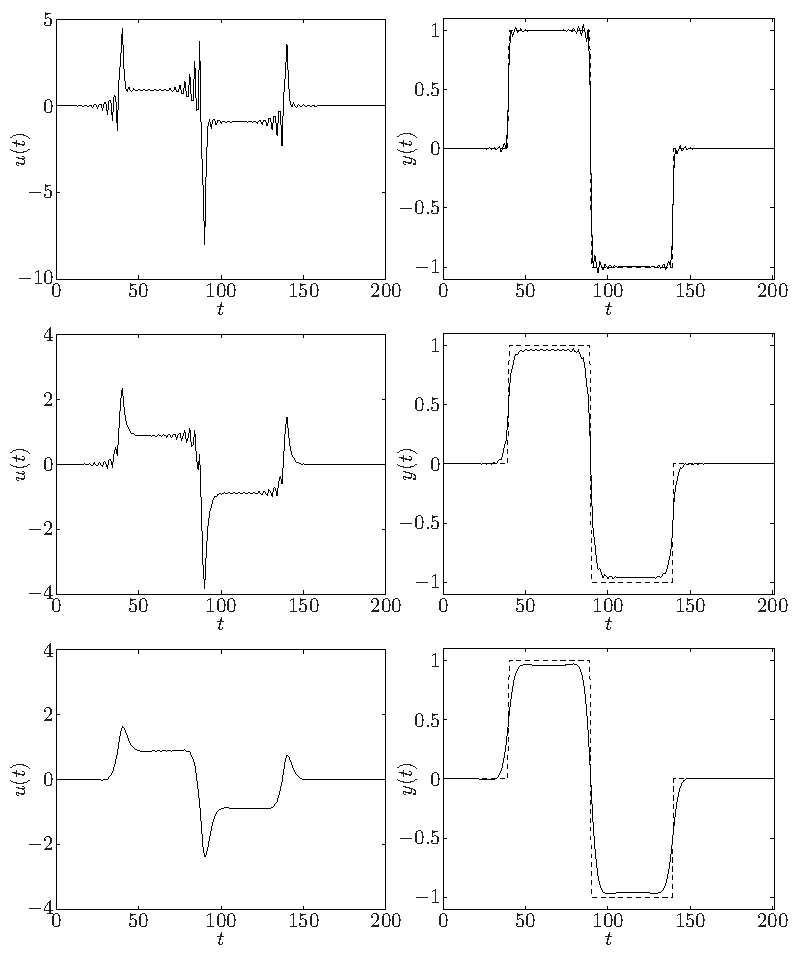
\includegraphics[width=.9\textwidth]{ch06-06.pdf}
\caption*{图6.6\quad 三组正则化参数下的最优输入（左）及相应输出（右）。$\delta$ 对应输入变化，$\eta$ 对应输入大小。右侧各图中的虚线是期望输出 $y_{\rm des}$。第一行：$\delta=0$、$\eta=0.005$；第二行：$\delta=0$、$\eta=0.05$；最后一行：$\delta=0.3$、$\eta=0.05$。}
\end{figure}

% Source PDF page 324 (printed p. 310)
改变参数 $\gamma$，就能描绘 $\norm{Ax-b}_2$ 与 $\norm x_1$ 之间的最优权衡曲线；它近似表示 $\norm{Ax-b}_2$ 与向量 $x$ 的稀疏程度或基数 $\operatorname{card}(x)$（即非零元素数）之间的最优权衡曲线。问题 (6.11) 可以改写为 SOCP 并求解。

\begin{origexample}{6.4}
\emph{回归向量选择问题。}给定矩阵 $A\in\R^{m\times n}$，其各列是候选回归向量；还有向量 $b\in\R^m$，要用 $A$ 的 $k<n$ 列的线性组合拟合它。问题是选择所用的 $k$ 个回归向量以及相应系数。可写成
\[\begin{array}{ll}\text{最小化}&\norm{Ax-b}_2\\\text{约束条件}&\operatorname{card}(x)\le k.\end{array}\]
一般而言，这是一个困难的组合问题。

一种直接方法是逐一检查 $x$ 的所有具有 $k$ 个非零元素的稀疏模式。固定稀疏模式后，可通过最小二乘问题求最优 $x$，即最小化 $\norm{\widetilde A\widetilde x-b}_2$，其中 $\widetilde A$ 是保留与该模式对应的列得到的 $A$ 的子矩阵，$\widetilde x$ 是由 $x$ 的非零分量构成的子向量。对全部 $n!/[k!(n-k)!]$ 种含 $k$ 个非零元素的稀疏模式，都进行这项计算。

一种良好启发式方法，是对不同 $\gamma$ 求解问题 (6.11)，找出使解满足 $\operatorname{card}(x)=k$ 的最小 $\gamma$，随后固定这个稀疏模式，寻找使 $\norm{Ax-b}_2$ 最小的 $x$。

图6.7给出一个数值例子，其中 $A\in\R^{10\times20}$、$x\in\R^{20}$、$b\in\R^{10}$。虚线上的圆圈是 $\operatorname{card}(x)$（纵轴）与残差 $\norm{Ax-b}_2$（横轴）之间权衡的全局 Pareto 最优值。对每个 $k$，均按上述方法枚举具有 $k$ 个非零元素的全部稀疏模式，得到 Pareto 最优点。实线上的圆圈则来自启发式方法，采用不同 $\gamma$ 下问题 (6.11) 的解所具有的稀疏模式。注意，当 $\operatorname{card}(x)=1$ 时，启发式方法确实找到了全局最优解。

基追踪（第6.5.4节）还会用到这个想法。
\end{origexample}

\subsection{重构、平滑与去噪}
本节介绍上述双准则逼近问题的一个重要特例，并用例子说明不同正则化方法的表现。重构问题从一个以向量 $x\in\R^n$ 表示的信号出发。系数 $x_i$ 对应某个时间函数在等间距点上的取值（用信号处理术语，就是采样值）。通常假设信号不会变化太快，也就是一般有 $x_i\approx x_{i+1}$。（本节考虑一维信号，如音频信号；同样的思想也适用于二维或更高维信号，如图像或视频。）
